\clearpage
\subsection{Jet background}
\label{FRsec}

The jet background is the smallest of the significant SM backgrounds considered in this search. The primary components of the jet background are: di-jet events, where both jets have passed electron ID criteria, \wjets\ events, where the W decays to an $e\nu$ pair and a jet passes the electron ID criteria and \phoJets\ events, where the photon and a jet passed electron ID criteria. The jet background is estimated using the `fake rate method' which is explained below.

\subsubsection{Jet to electron misidentification probability measurement}


The probability for a jet reconstructed as an electron to pass the HEEP ID selection, here after referred to as a `fake rate', is measured using data events triggered by single photon triggers.

The fake rate is measured in bins of $E_{T}^{HLT}$ and $\eta_{SC}$, where $E_{T}^{HLT}$ is the transverse energy of the electron as obtained by the HLT and $\eta_{SC}$ is the $\eta$ of the RECO supercluster of the electron w.r.t 0,0,0. The fake rate is relatively flat across the barrel but increases with increasing $\eta$ in the endcap. Therefore, while the barrel is one $\eta$ bin, the endcap is split into two $\eta$ bins.
Given the rate of change of the fake rate with $E_T$ and that the overall precision is not high, using RECO $E_T$ on a HLT $E_T$ parameterized function is not expected to have any significant effect.

The fake rate is measured with respect to an electron candidate passing both the fake rate pre-selection in table~\ref{tab:frPreSel} and the first leg of either the HLT\_DoubleEle33\_CaloIdL\_GsfTrkIdVL or HLT\_DoubleEle33\_CaloIdL\_MW trigger, with the exact trigger requirement being run dependent. There can be only one ECAL driven reconstructed electron with $E_{T}>10$~GeV and H/E$<0.15$ in the event to reduce contamination from \zee\ events. The fake rate is therefore simply the number of misidentified jets in this sample which then go on to pass the HEEP selection.

The number of misidentified jets in this sample is estimated using track isolation template for jets normalised to the observed N-1 track isolation distribution for each bin the fake rate is calculated in. The N-1 track isolation distribution is simply the track isolation distribution for electron candidates in the fake rate sample which pass the HEEP selection with the track isolation cut removed.

The distribution of the track isolation for jets is obtained by requiring the electron candidate to pass the H/E and calorimeter isolation cuts but fail at least one other cut.
In practice the cuts which it is possible for the electron candidate to fail are the \dEtaInSeed, \dPhiIn, and shower shape cuts.
The H/E and calorimeter isolation variables are strongly correlated with the track isolation variable and misidentified jets which pass these cuts will have a different track isolation distribution to misidentified jets which fail this cuts.

The jet track isolation template is then normalised to the observed N-1 track isolation distribution in the range of $10 < $Isol $p_{T}$ Tracks$ < 20$~GeV.
Any signal contamination in this region is small and is predicted to be a maximum of a few percent from Monte Carlo simulated events. To be clear, it is this feature that allows us to forget a signal template.

Then the prediction of the normalised jet template for the number electron candidates with Isol $p_{T}$ Tracks$ < 5$~GeV is taken as the number of misidentified jets passing HEEP selection.

To summarise the method, the number of jets passing HEEP ID is the number of events in the jet tracker isolation template below 5 GeV once that template has been normalised to observed N-1 track isolation distribution in a region where there are no signal events.
%The jet templates are further scrutinised in section~\ref{sec:trkIsoTemps}.

The measured fake rates in 2016 (2017) are shown in figure~\ref{fr:fig:heepFRV70VsEt_2016} (\ref{fr:fig:heepFRV70VsEt_2017}), together with simple fitted functions to allow the fake rate to be easier to apply in the analysis.
The fit parameters are summarised in table~\ref{fr:tab:heepFRV70}.
A 50\% uncertainty on the method is assumed and this seems cover deviations from the arbitrarily chosen fits.
More details can be found in \cite{CMS-AN-2016-404}.


\begin{table}
\begin{center}
\begin{tabular}{|c|c|c|} \hline
variable & barrel  & endcap   \\\hline
\sigmaIEtaIEta & $<$0.013 & $<$0.034 \\
H/E & $<$0.15 & $<$0.10 \\
nr. missing hits & $<=1$ & $<=1$ \\
$|$dxy$|$ & $<0.02$ & $<0.05$ \\\hline
\end{tabular}
\caption{The selection requirements for the starting point of the fake rate calculation.}
\label{tab:frPreSel}
\end{center}
\end{table}

\begin{figure}[b]
  \begin{center}
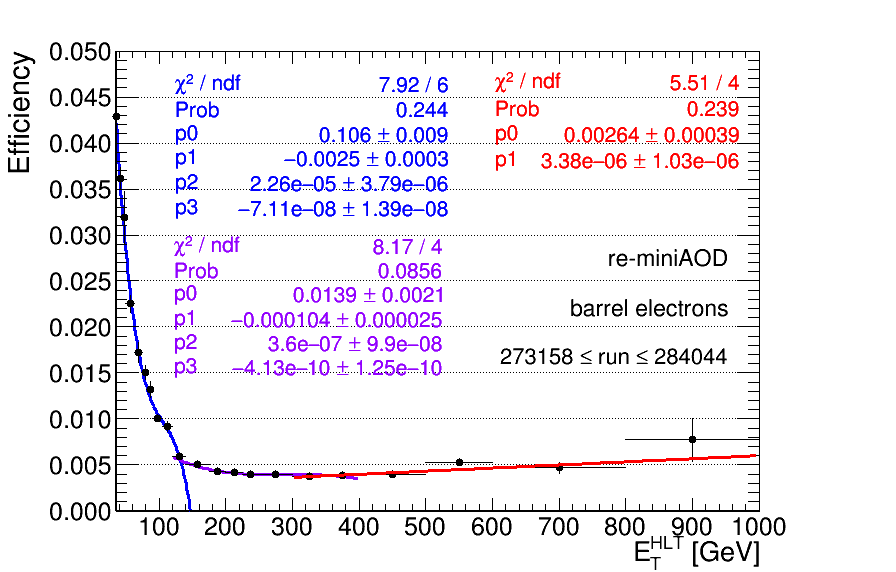
\includegraphics[width=0.47\linewidth,angle=0]{figures/Zprime/2016/fakeRates/frEBGSFixed.png}
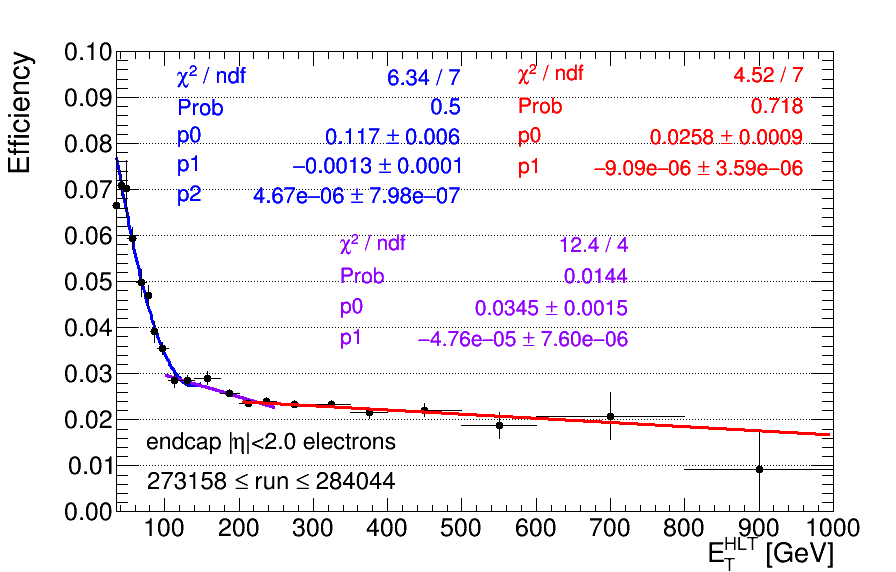
\includegraphics[width=0.47\linewidth,angle=0]{figures/Zprime/2016/fakeRates/frEELowVsEt.png}
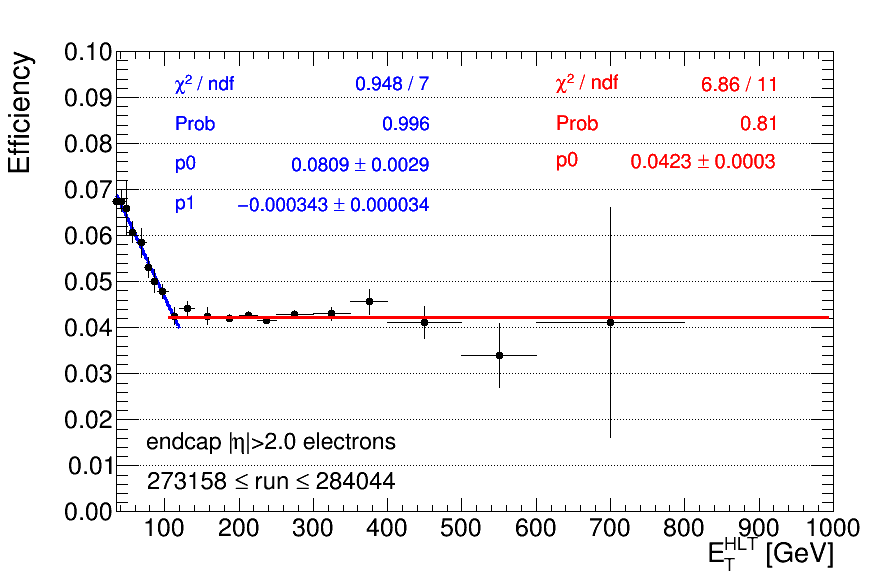
\includegraphics[width=0.47\linewidth,angle=0]{figures/Zprime/2016/fakeRates/frEEHighVsEt.png}
    \caption{The measured HEEP ID fake rate vs $E_T$ for the barrel region (top left), the endcap low $\eta$ region (top right) and the endcap high $\eta$ region (bottom) in 2016.}
       \label{fr:fig:heepFRV70VsEt_2016}
  \end{center}
\end{figure}

\begin{figure}[b]
  \begin{center}
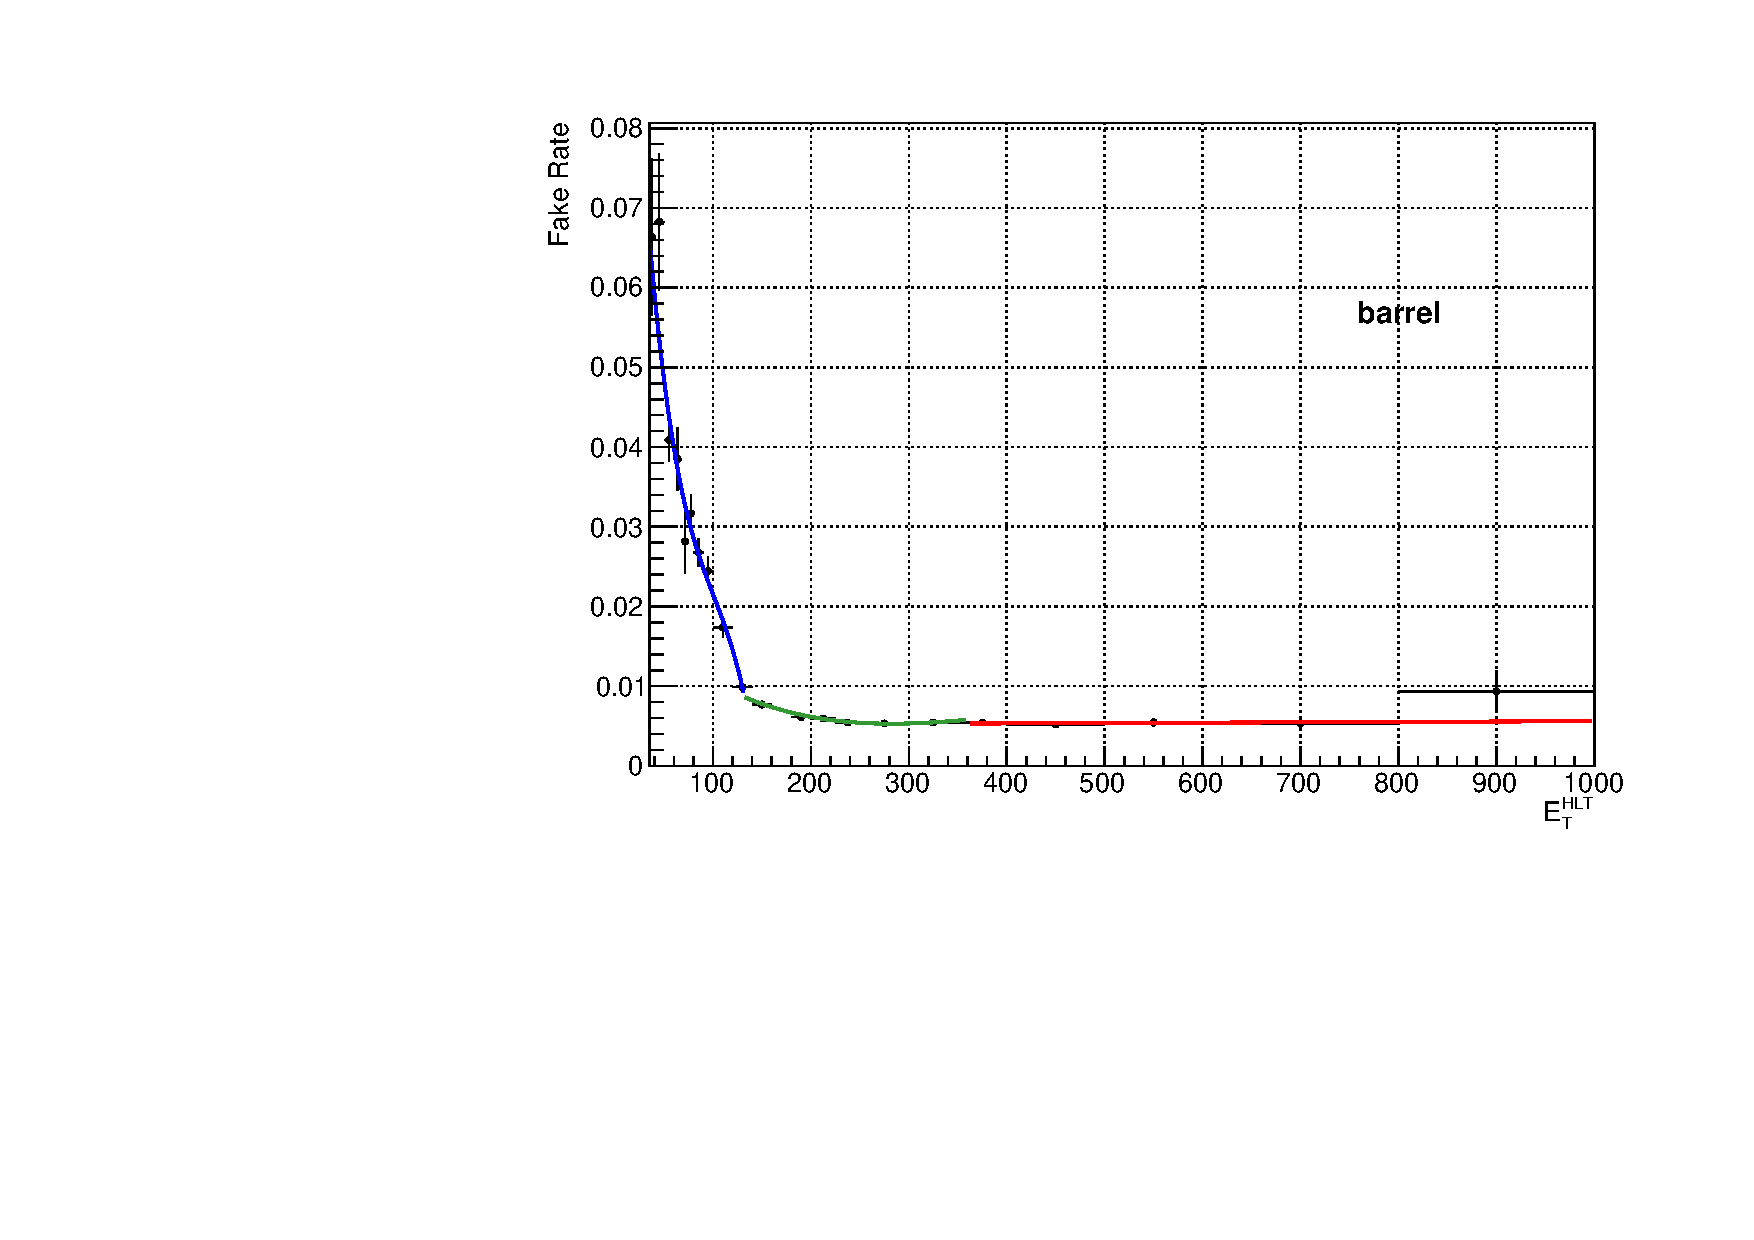
\includegraphics[width=0.47\linewidth,angle=0]{figures/Zprime/2017/fakeRates/FakeRate_Barrel.pdf}
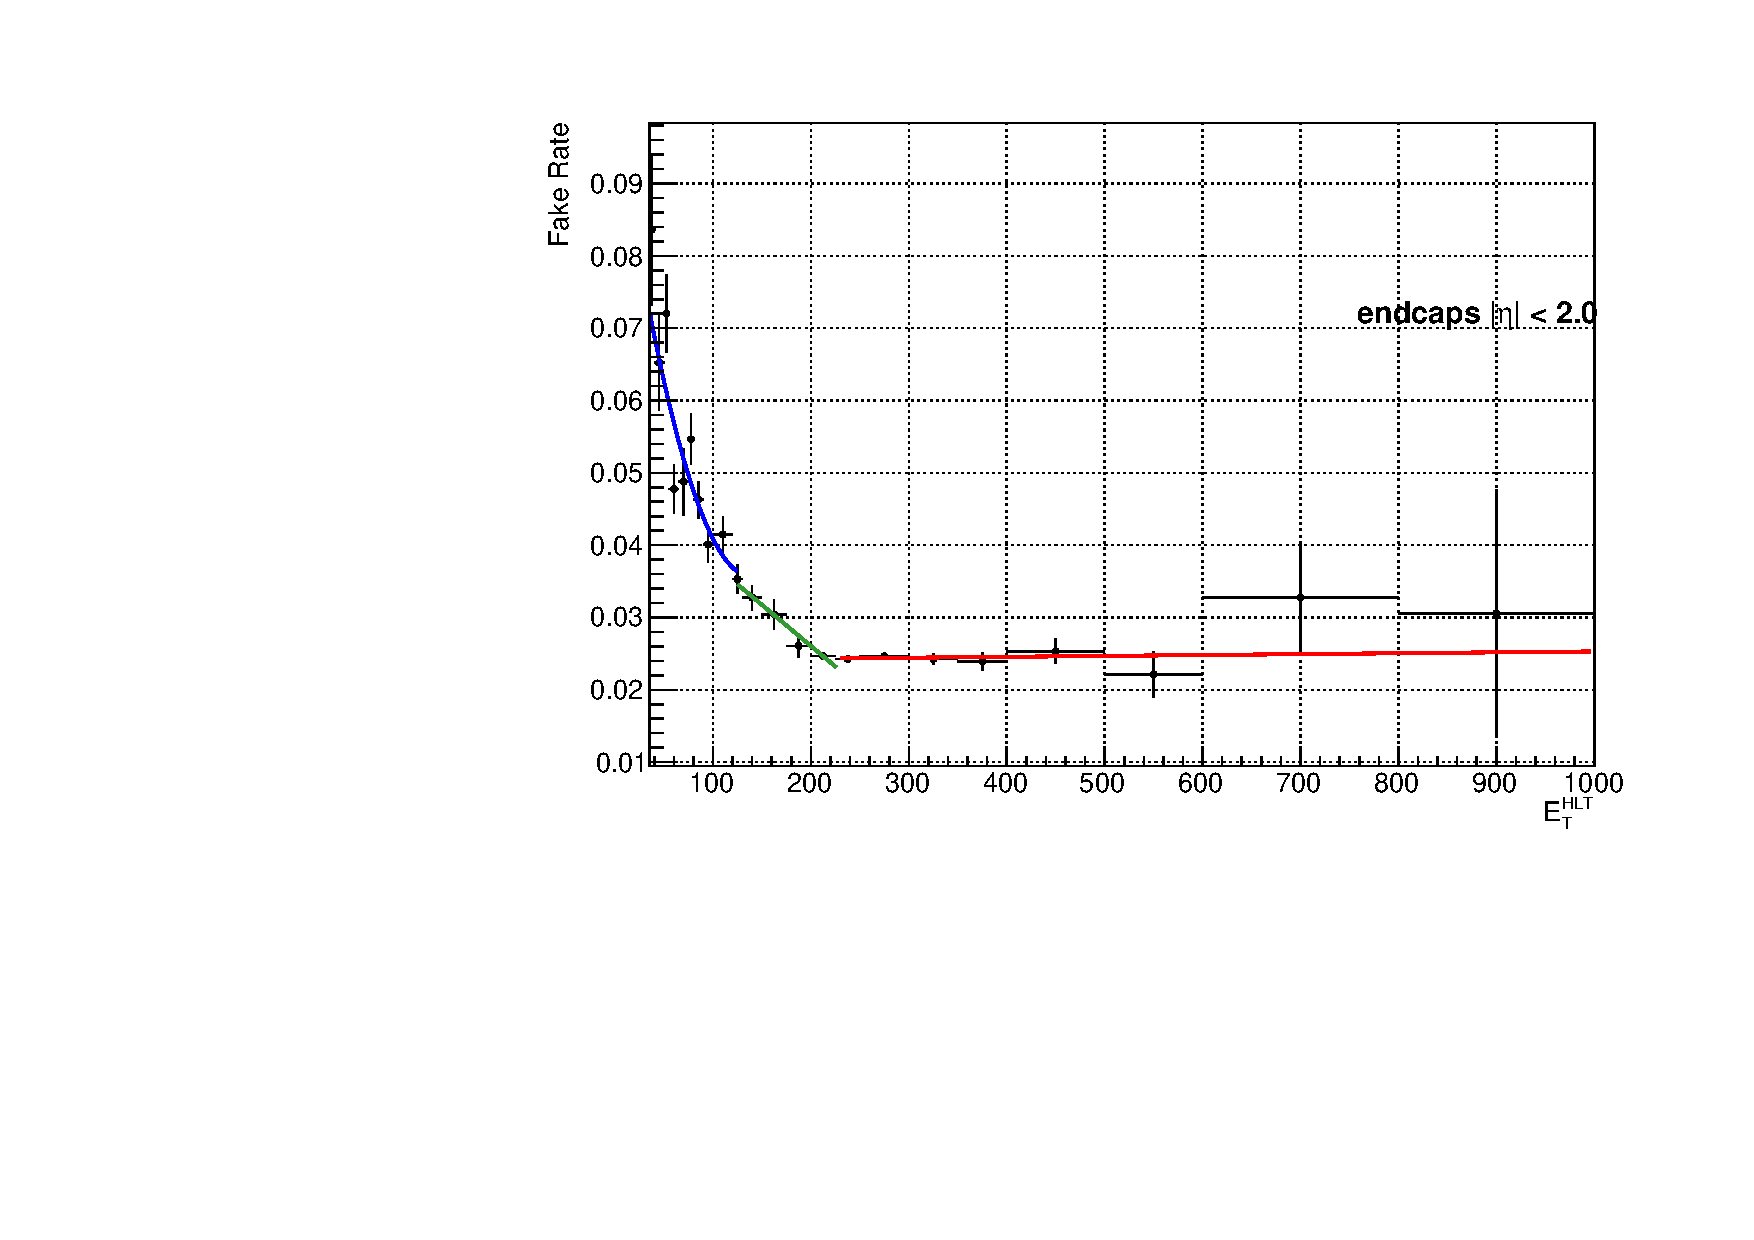
\includegraphics[width=0.47\linewidth,angle=0]{figures/Zprime/2017/fakeRates/EndCap_Eta_less2.pdf}
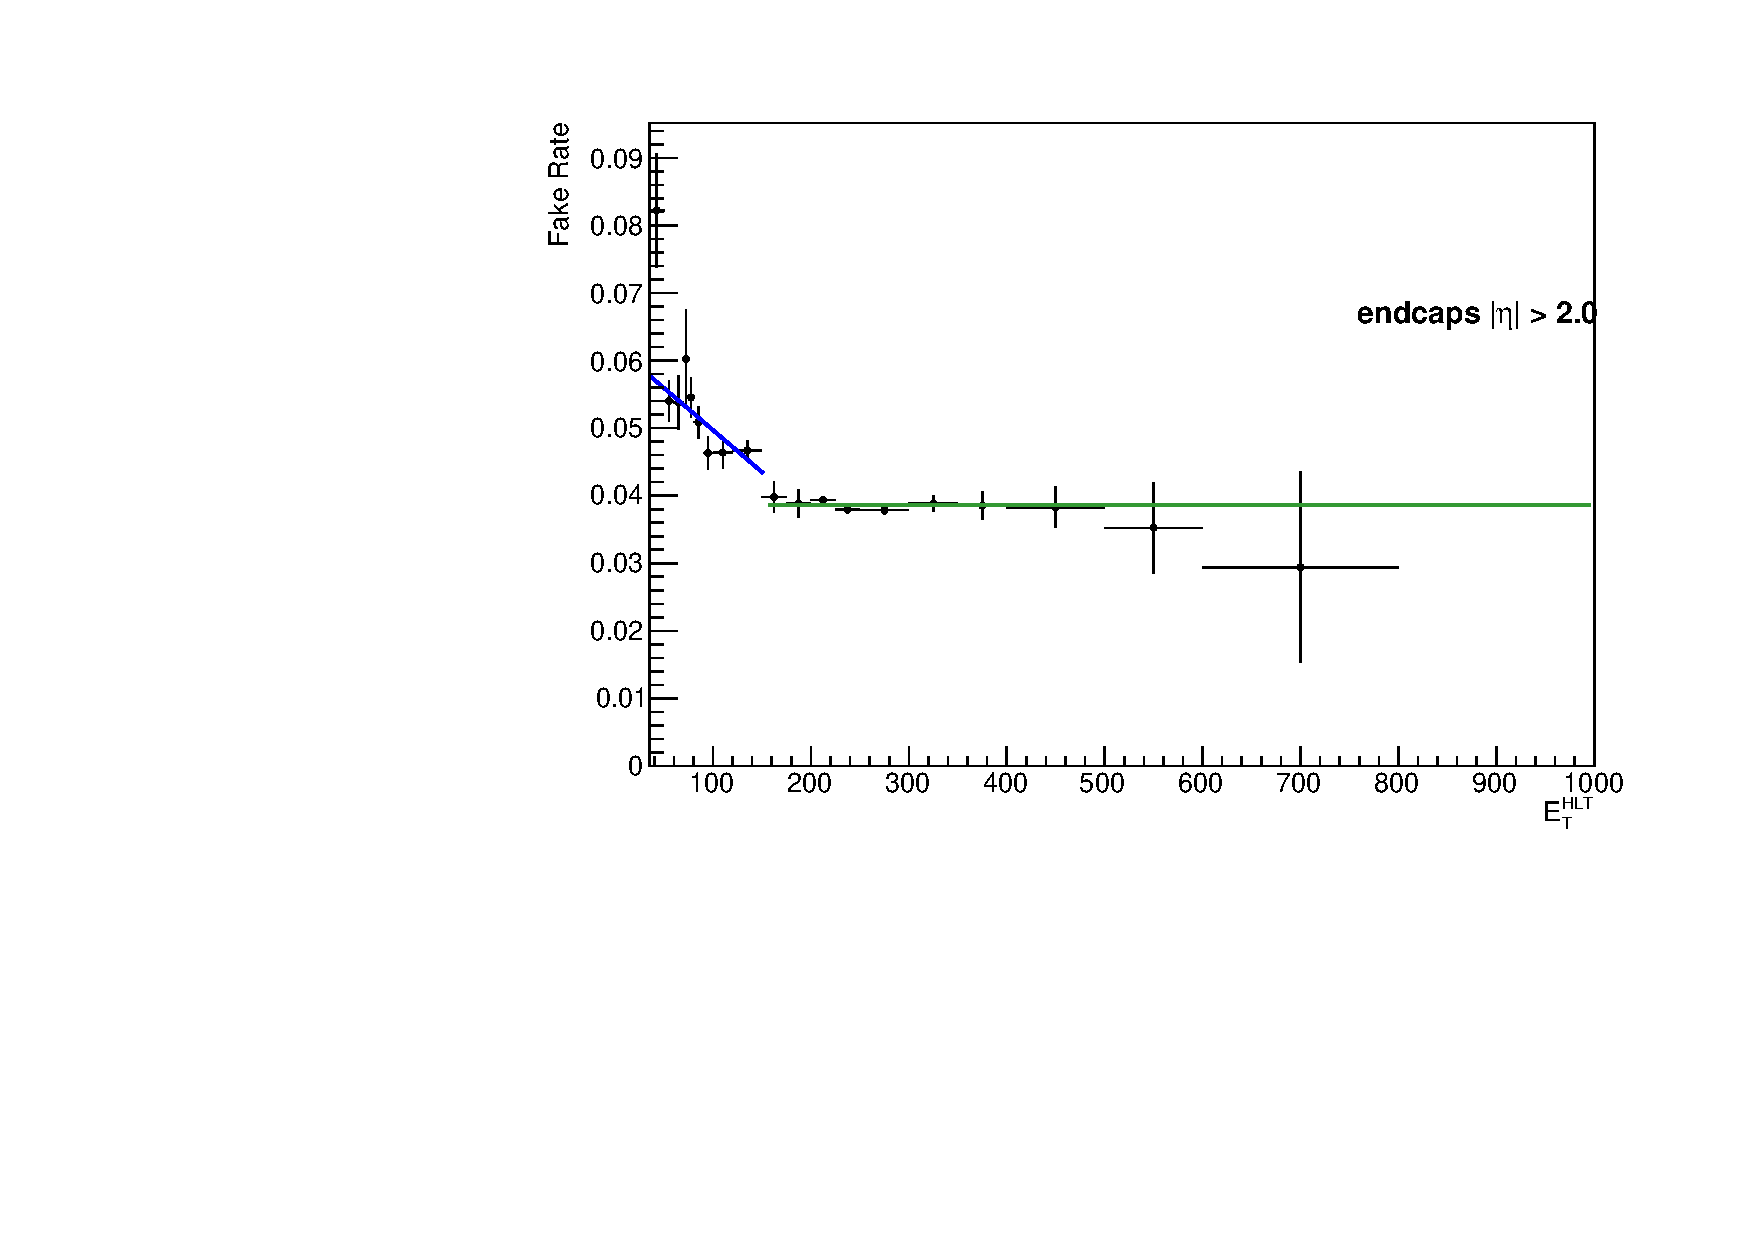
\includegraphics[width=0.47\linewidth,angle=0]{figures/Zprime/2017/fakeRates/Ext_Endcap.pdf}
    \caption{The measured HEEP ID fake rate vs $E_T$ for the barrel region (top left), the endcap low $\eta$ region (top right) and the endcap high $\eta$ region (bottom) in 2017.}
       \label{fr:fig:heepFRV70VsEt_2017}
  \end{center}
\end{figure}

\begin{table}
\begin{center}
\resizebox{\linewidth}{!}{
\begin{tabular}{|c|c|c|c|} \hline
Year &region                 & $E_T$ range (GeV)              & functional form  \\\hline
\multirow{8}{*}{2016}&\multirow{3}{*}{barrel}& $35.0 \leq E_{T} < 131.6$ GeV  &$ 0.106 - 0.0025 \times E_{T} + 2.26\times 10^{-5} \times E_{T}^{2} - 7.11\times 10^{-8} \times E_{T}^{3} $\\ \cline{3-4}
&                       &$131.6 \leq E_{T} < 359.3$ GeV  &$ 0.0139 - 0.000104 \times E_{T} + 3.6\times 10^{-7} \times E_{T}^{2} - 4.13\times 10^{-10} \times E_{T}^{3}$\\ \cline{3-4}
&                       & $E_{T} \geq 359.3$ GeV         &$ 0.00264 + 3.38\times 10^{-6} \times E_{T} $\\ \cline{2-4}
&\multirow{3}{*}{endcap $|\eta|<2.0$}  & $35.0 \leq E_{T} < 122.0$ GeV  & $ 0.117 - 0.0013 \times E_{T} + 4.67\times 10^{-6} \times E_{T}^{2} $\\ \cline{3-4}
&                                      & $122.0 \leq E_{T} < 226.3$ GeV & $ 0.0345 - 4.76\times 10^{-5} \times E_{T} $\\ \cline{3-4}
&                                      & $E_{T} \geq 226.3$ GeV         & $ 0.0258 - 9.09\times 10^{-6} \times E_{T} $\\ \cline{2-4}
&\multirow{2}{*}{endcap $|\eta|>2.0$}  & $35.0 \leq E_{T} < 112.5$ GeV  & $ 0.0809 - 0.000343 \times E_{T} $\\ \cline{3-4}
&                                      & $E_{T} \geq 112.5$ GeV         & $ 0.0423 $\\\hline
\multirow{8}{*}{2017}&\multirow{3}{*}{barrel}& $35.0 \leq E_{T} < 131.6$ GeV  & $ 0.140 - 0.0029 \times E_{T} + 2.56\times 10^{-5} \times E_{T}^{2} - 8.48\times 10^{-8} \times E_{T}^{3} $\\ \cline{3-4}
&                       & $131.6 \leq E_{T} < 359.3$ GeV & $ 0.020 - 0.00013 \times E_{T} + 3.50\times 10^{-7} \times E_{T}^{2} - 2.90\times 10^{-10} \times E_{T}^{3} $\\ \cline{3-4}
&                       & $E_{T} \geq 359.3$ GeV         & $ 0.00514 + 4.73\times 10^{-7} \times E_{T} $\\\cline{2-4}
&\multirow{3}{*}{endcap $|\eta|<2.0$}   & $35.0 \leq E_{T} < 125.0$ GeV  & $ 0.1012 - 0.00094 \times E_{T} + 3.37\times 10^{-6} \times E_{T}^{2} $\\ \cline{3-4}
&                                       & $125.0 \leq E_{T} < 226.3$ GeV & $ 0.0488  - 11.37\times 10^{-5} \times E_{T} $\\ \cline{3-4}
&                                       & $E_{T} \geq 226.3$ GeV         & $ 0.0241 - 1.24 \times 10^{-6} \times E_{T} $\\\cline{2-4}
&\multirow{2}{*}{endcap $|\eta|>2.0$}   & $35.0 \leq E_{T} < 152.$ GeV   & $ 0.0622 - 0.00012 \times E_{T} $\\ \cline{3-4}
&                                       & $E_{T} \geq 152.$ GeV          & $ 0.0387 $\\\hline

\end{tabular}}
\caption{The functional approximation of the measured fake rate for HEEP electrons in the barrel and endcap vs $E_T$.}
\label{fr:tab:heepFRV70}

\end{center}
\end{table}

%\subsubsection{Scrutiny of the Tracker Isolation Templates}
%\label{sec:trkIsoTemps}
%There is a substantial contamination of real electrons in the fake rate sample and the measurement depends on the jet isolation template to correct for this.
%Therefore it is vital to show that obtained template is a good approximation to the true jet tracker isolation distribution for jets misidentified as HEEPV7.0 electrons.
%Section~\ref{sec:appendix_fr_temps} in Appendix~\ref{sec:appendix_fr} has further details on this, including all the track isolation distributions for all the bins the fake rate is calculated in.
%
%An example of the tracker isolation distribution in a bin is shown in figure~\ref{fr:fig:frTempExample} for the three $\eta$ regions.
%To further scrutinise the accuracy of the jet template, an electron template is generated from Drell-Yan Monte Carlo and the two templates are fitted to the data.
%The electron template is simply the N-1 track isolation distribution in the $E_T$, $\eta$ appropriate bin. To be clear, this is only done to help us decide if the jet templates are reasonable, due to the good separation of electrons and jets by tracker isolation, no electron template is required to measure the fake rate.
%
%As can be seen from figure~\ref{fr:fig:frTempExample}, there is excellent separation between electrons and jets.
%Over all there is an acceptable agreement between the data and the two templates.
%Below 20 GeV, the maximum deviations are in the 10-20\% range and there are no persistent trends in the agreement across the different $E_T$, $\eta$ bins.
%However, as figure~\ref{fr:fig:frTempExample} also shows, in higher $E_T$ bins, the jet template falls slower than the data, leading to an over prediction for values of tracker isolation greater then 20~GeV.
%This effect is smaller in the endcap. It implies that there is some small correlation between the tracker isolation variable and the shower shape, \dEtaInSeed, and \dPhiIn cuts, with jets having passed those cuts being less likely to have a very high value of tracker isolation.
%
%The concern with the jet template is not that it models high values of tracker isolation correctly but the low values correctly, specifically the region from 0 to 5 GeV must be trusted.
%In most $E_T$, $\eta$ bins the tracker isolation agrees fits well to the templates below 20 GeV, even in the 5-10 GeV bin which has little electron contribution.
%Therefore it gives confidence that the 0-5 GeV jet template is accurate.
%From comparing deviations at high tracker isolation, if the measured jet template is distorted from the true jet track isolation distribution, this is likely to be not more than 20-30\% which, given the target accuracy of the method of 50\%, is not a problem.
%
%\begin{figure}[b]
%  \begin{center}
%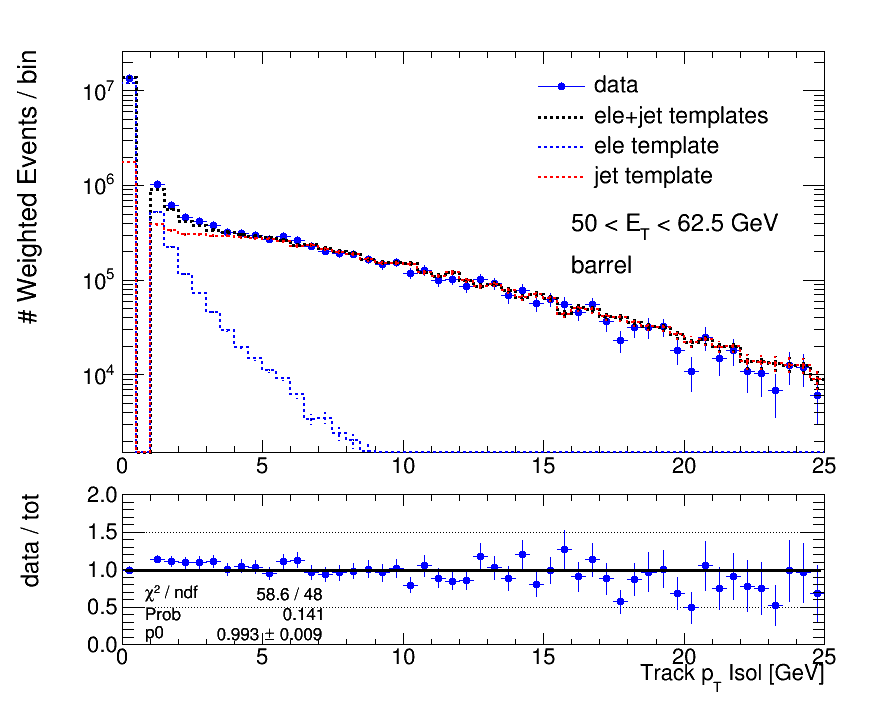
\includegraphics[width=0.49\linewidth,angle=0]{fig/fig_fakeRates/frTempEB0p5GeVSimpleFitEBEt50To62p5.png}
%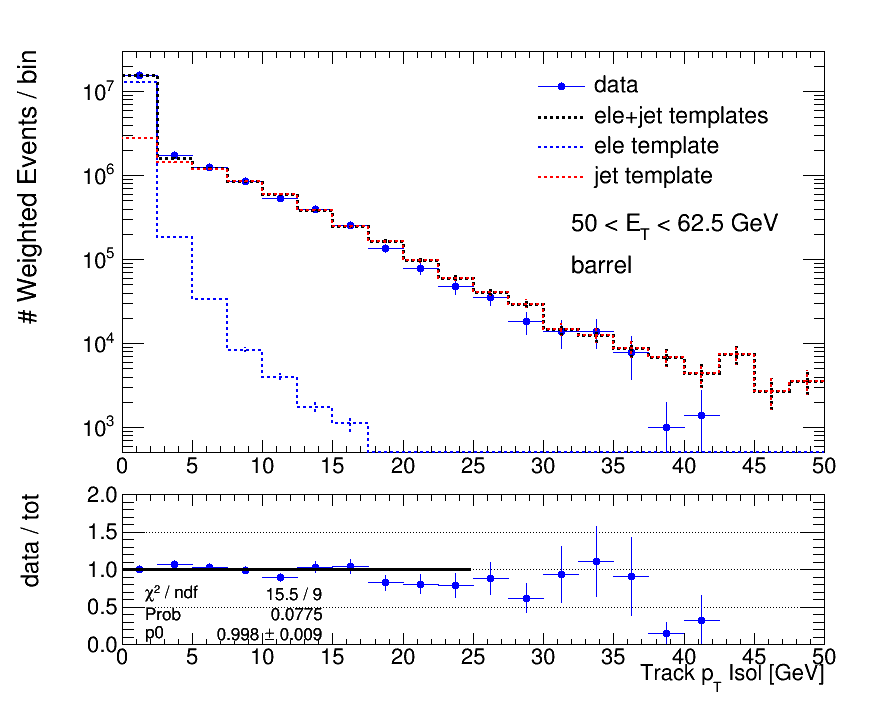
\includegraphics[width=0.49\linewidth,angle=0]{fig/fig_fakeRates/frTempEB2p5GeVSimpleFitEBEt50To62p5.png}
%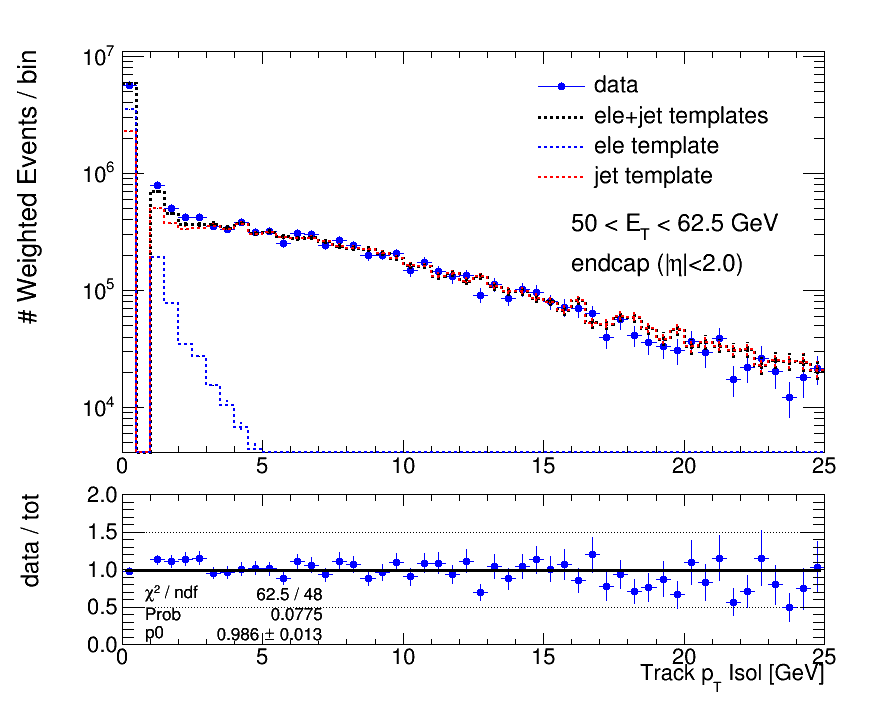
\includegraphics[width=0.49\linewidth,angle=0]{fig/fig_fakeRates/frTempEELow0p5GeVSimpleFitEELowEt50To62p5.png}
%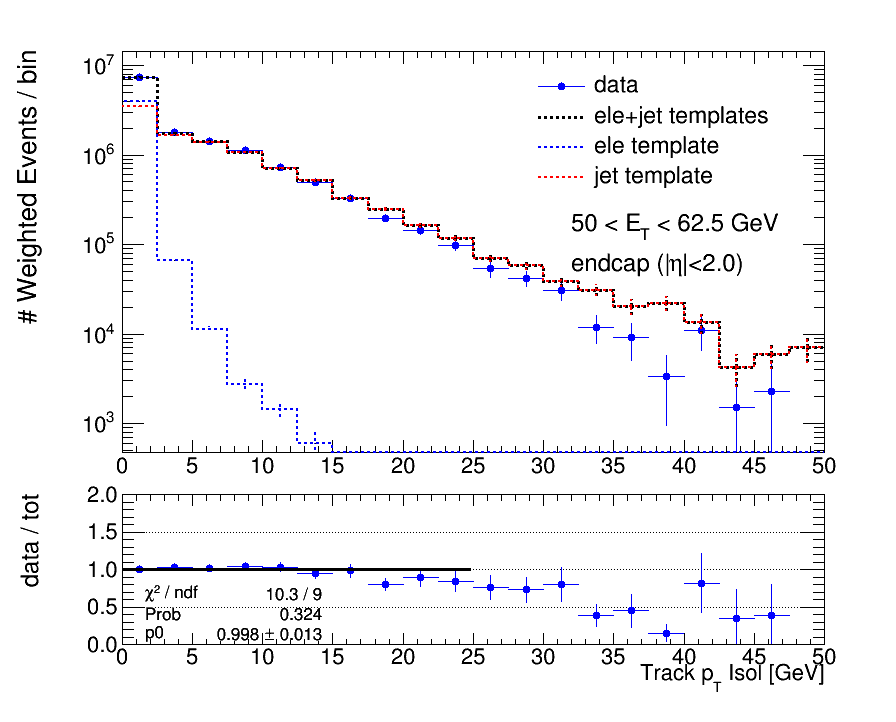
\includegraphics[width=0.49\linewidth,angle=0]{fig/fig_fakeRates/frTempEELow2p5GeVSimpleFitEELowEt50To62p5.png}
%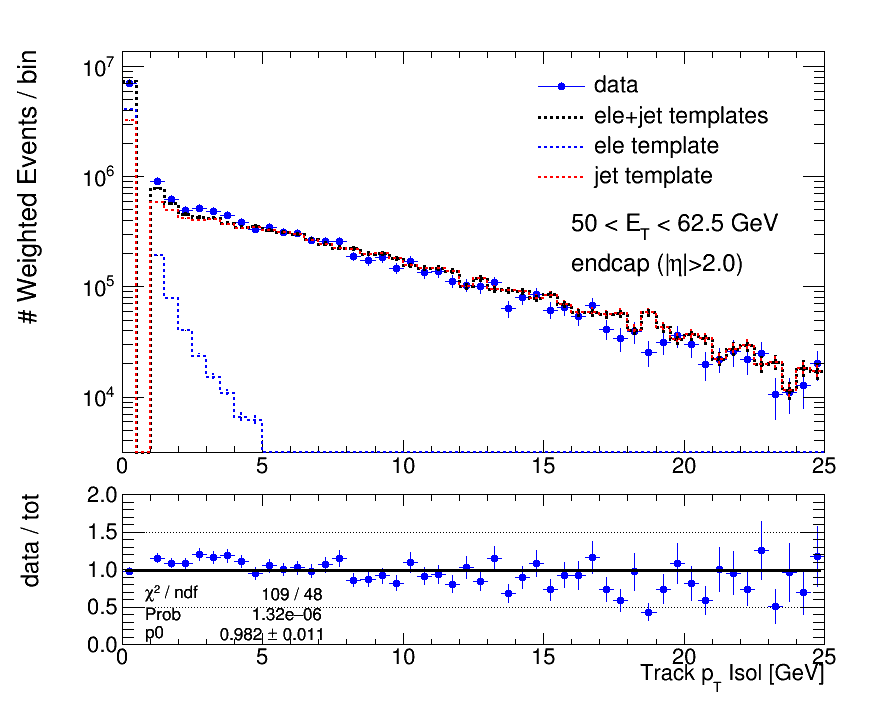
\includegraphics[width=0.49\linewidth,angle=0]{fig/fig_fakeRates/frTempEEHigh0p5GeVSimpleFitEEHighEt50To62p5.png}
%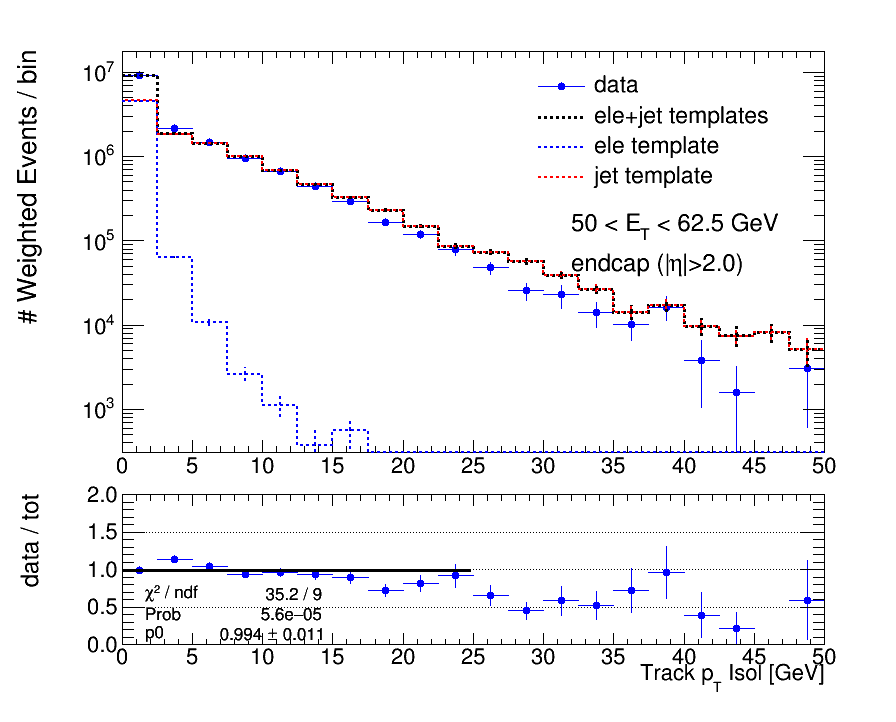
\includegraphics[width=0.49\linewidth,angle=0]{fig/fig_fakeRates/frTempEEHigh2p5GeVSimpleFitEEHighEt50To62p5.png}
%    \caption{An example fit of the electron and jet templates to the observed track isolation in 0.5 GeV bins (left) and 2.5 GeV bins (right) for electron candidates passing all but the track isolation cut. Note, this is for visual verification only, the electron template is not used when estimating the number of jets in this distribution.  }
%       \label{fr:fig:frTempExample}
%  \end{center}
%\end{figure}
%



\subsubsection{Jet mass spectrum estimates}

The jet background is estimated by selecting electron pairs passing the primary analysis trigger with one electron passing the HEEP selection and one electron passing the fake rate (FR) pre-selection in table~\ref{tab:frPreSel} but failing the HEEP selection. This is referred to as the 1FR estimate.
The events are then weighted by $FR/(1-FR)$ where $FR$ is the $E_T$ and $\eta$ appropriate fake rate for the electron failing the HEEP selection. In the case of more than one electron pair in the same event satisfying these conditions, all valid pairs are allowed to enter the estimation. There is a residual contamination of the \zee\ events which is corrected for by directly subtracting off the MC estimate.% although this is only significant at the Z peak.

The 1FR estimate includes the background from \wjets, \phoJets\ and di-jets but due to combinatorial effects, the 1FR estimate overestimates the di-jet contribution by a factor 2. The di-jet component can be estimated by selecting electron pairs where both electrons pass the FR pre-selection but fail the HEEP selection, again selected using the primary analysis trigger. This is referred to as the 2FR estimate. These events are weighted by $FR_{1}/(1-FR_{1}) \times FR_{2}/(1-FR_{2})$ where $FR_{1}$ ($FR_{2}$) is the $E_T$ and $\eta$ appropriate fake rate for the first (second) electron. This estimate is then subtracted off the 1FR estimate to estimate the total jet background without any double counting.

Due to fake rate measurement uncertainties and statistical effects, the 2FR estimate can sometimes be greater than half the 1FR estimate. This implies that the entirety of the 1FR estimate is from di-jets and therefore the true estimate of the di-jet background is simply 50\% of its value. Therefore the 1FR estimate can only be reduced to a minimum of 50\% of its uncorrected value.

The fake rate is tested using the invariant mass of two electrons passing HEEP ID and both in endcap region. Because there are more jets in endcap comparing with barrel region. The results are shown in Figure \ref{fig:Mee_endcap_endcap} (the uncertainty band is explained in \ref{sec:results}) and one can see the data and MC agree within uncertainty.

\begin{figure}[b]
  \begin{center}
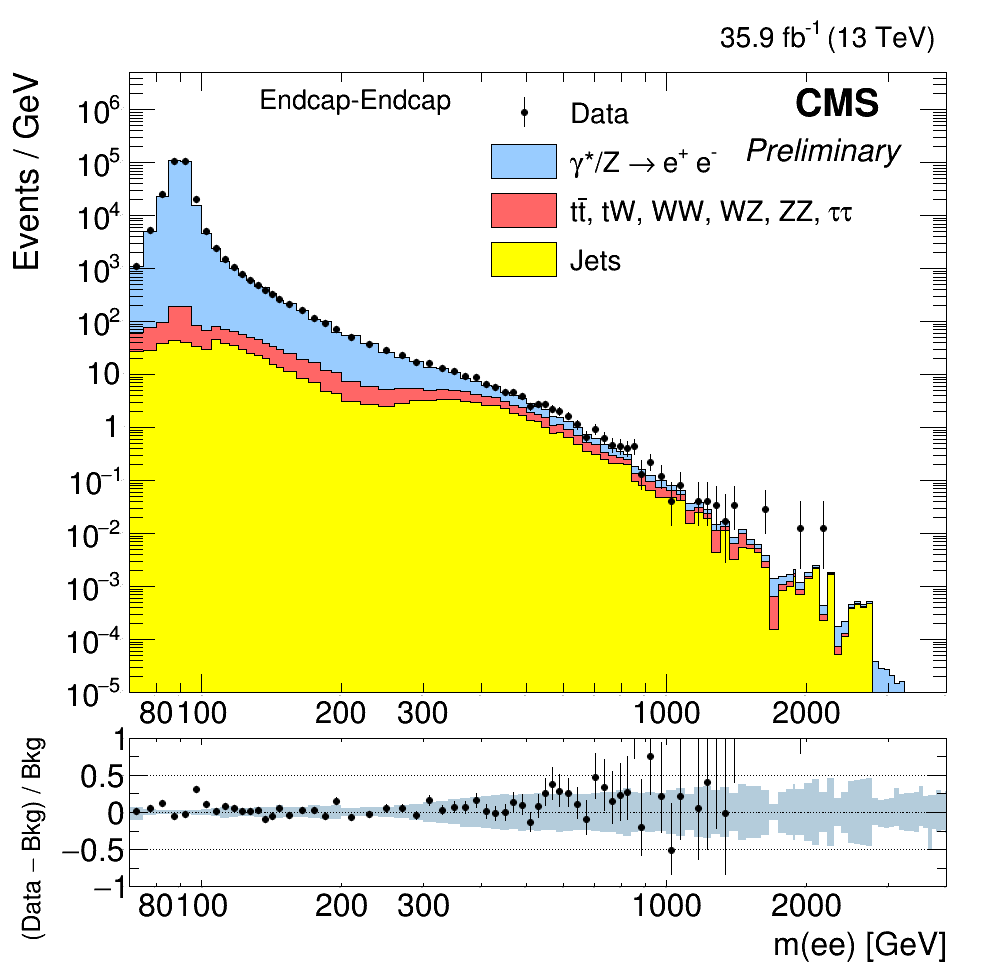
\includegraphics[width=0.47\linewidth,angle=0]{figures/Zprime/2016/mass/massHistEEEE.png}
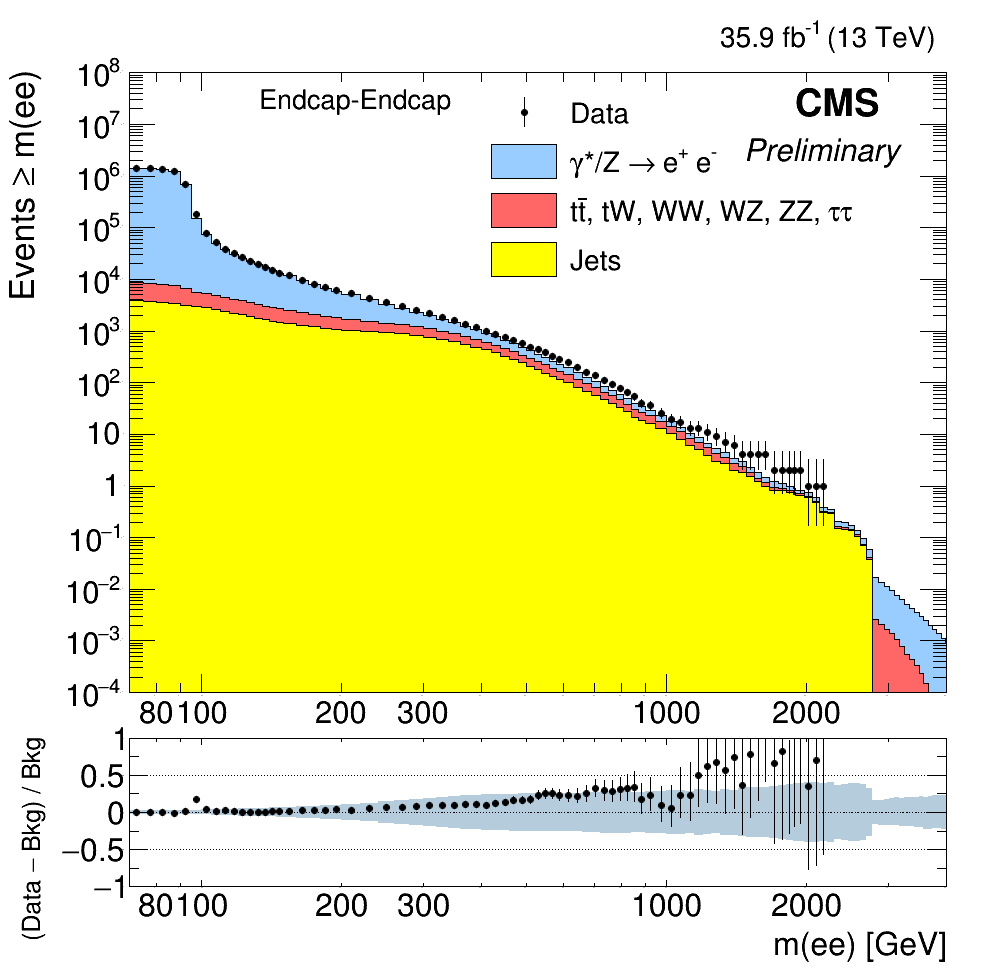
\includegraphics[width=0.47\linewidth,angle=0]{figures/Zprime/2016/mass/cMassHistEEEE.png}
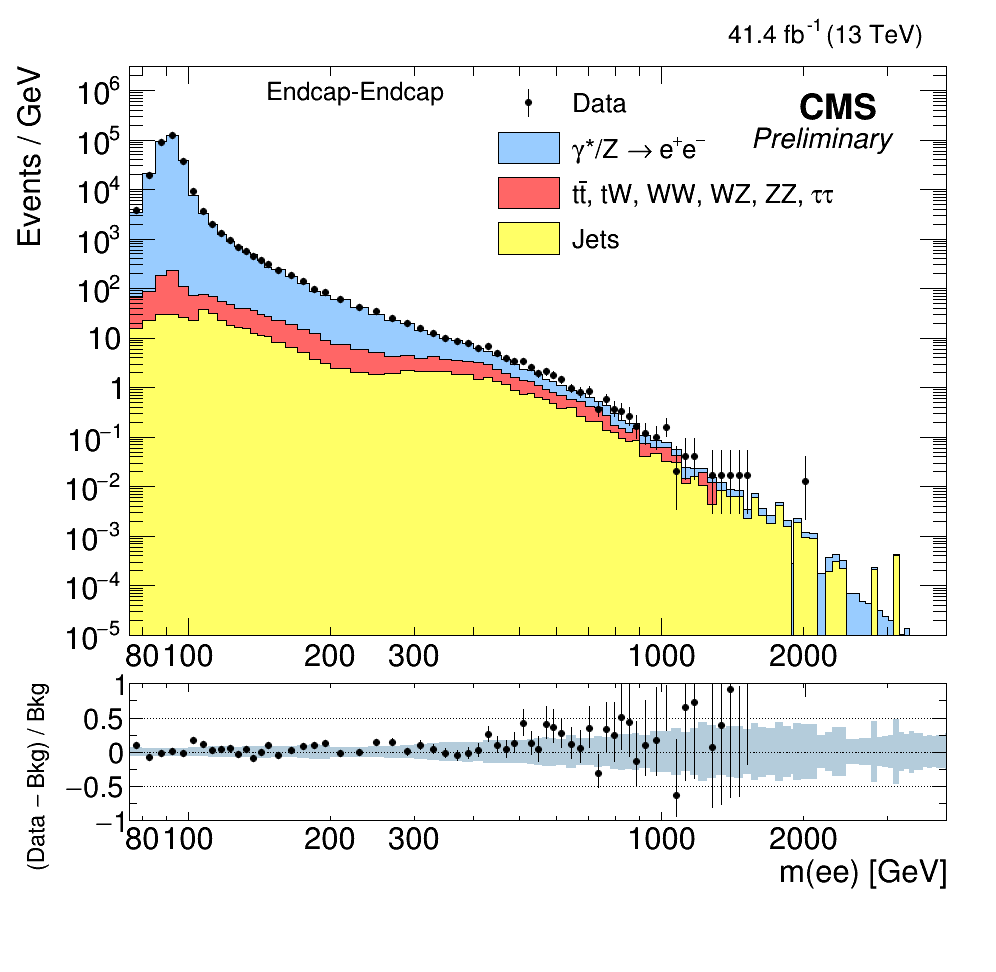
\includegraphics[width=0.47\linewidth,angle=0]{figures/Zprime/2017/mass/massHistEEEE.png}
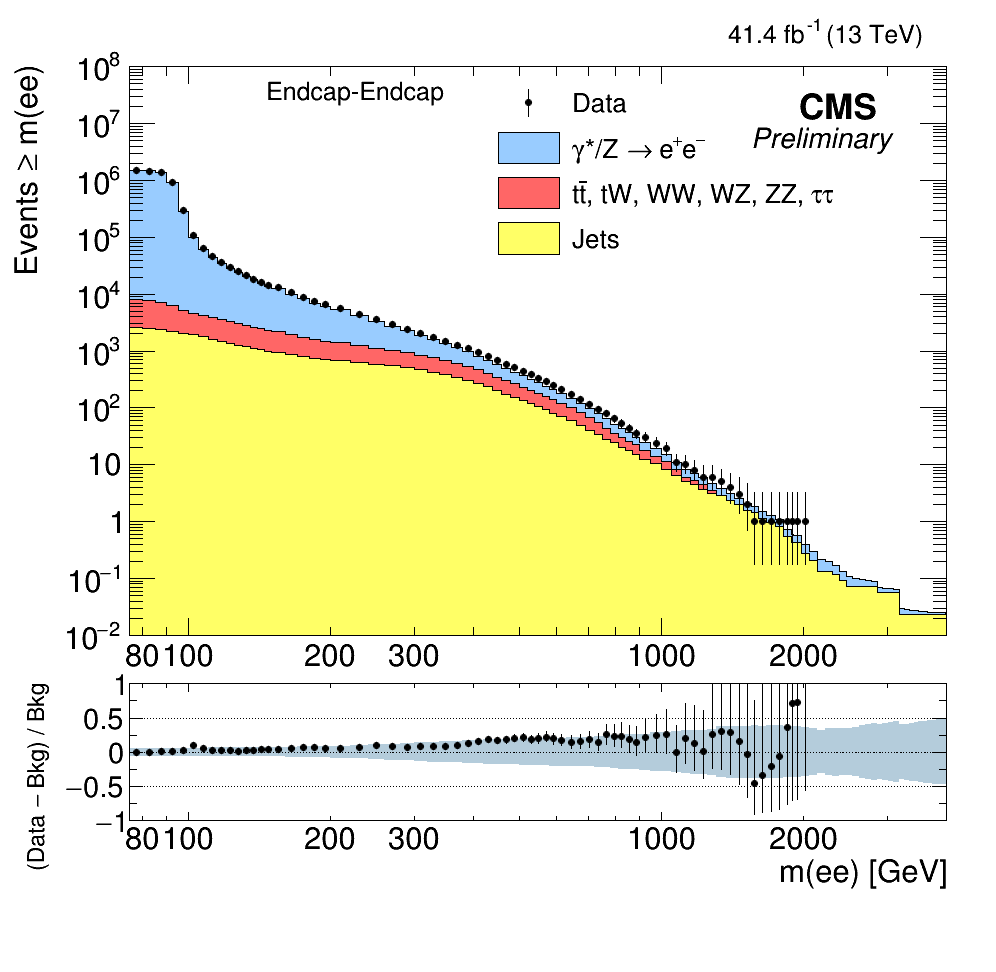
\includegraphics[width=0.47\linewidth,angle=0]{figures/Zprime/2017/mass/cMassHistEEEE.png}
    \caption{The dielectron mass spectrum (left) and the cumulated distribution (right) for both electrons in endcap in 2016 (top) and 2017 (bottom).}
       \label{fig:Mee_endcap_endcap}
  \end{center}
\end{figure}

